\chapter{Menginputkan File Excel Ke Dalam Database APEX}

\begin{enumerate}
\item[1]Buat Data mahasiswa di excel dengan format .xlsx.
    \begin{figure}[!htbp]
    \begin{center}
    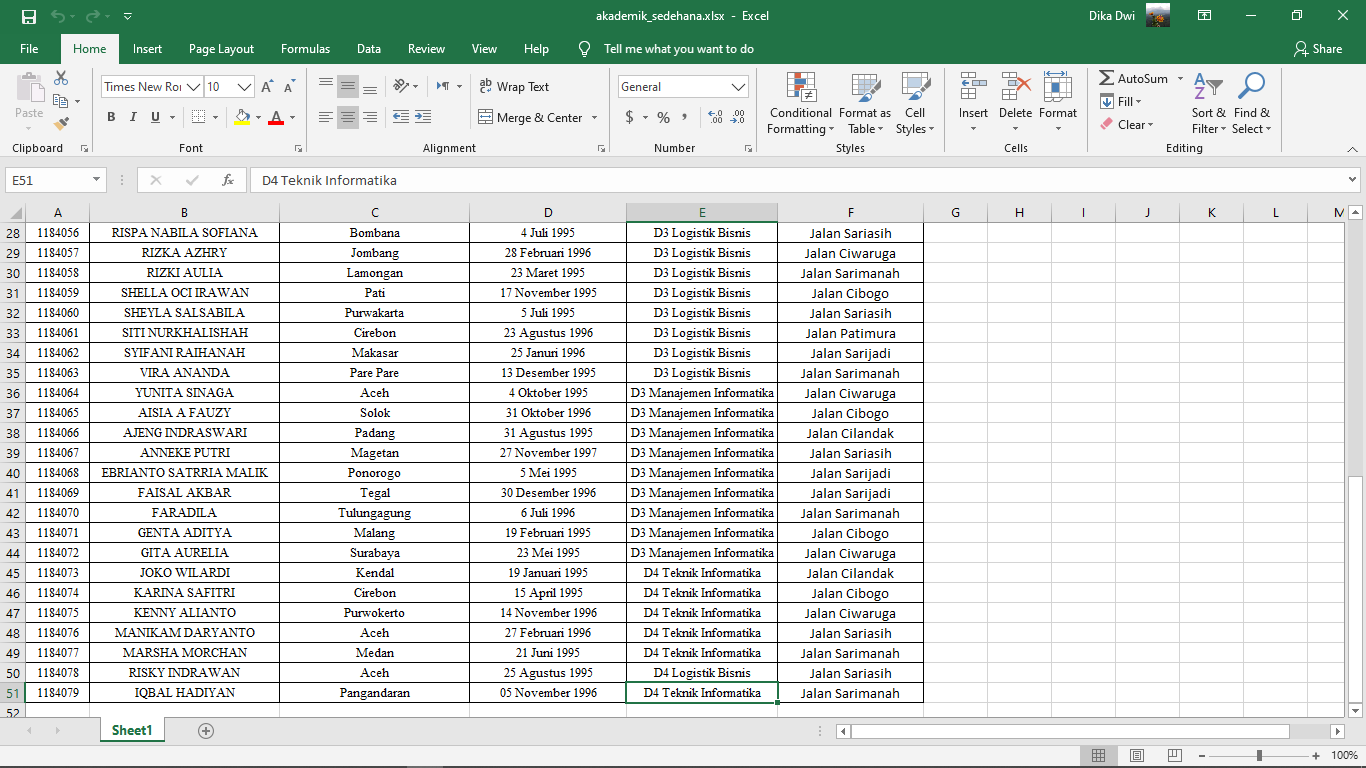
\includegraphics[scale=0.2]{figures/0.png}
    \caption{\textit{Contoh Isi File Tabel data Mahasiswa}}
    \end{center}   
\item[2]Masuk ke dalam Oracle APEX online Dan klik Request A Workspace.

    \begin{center}
    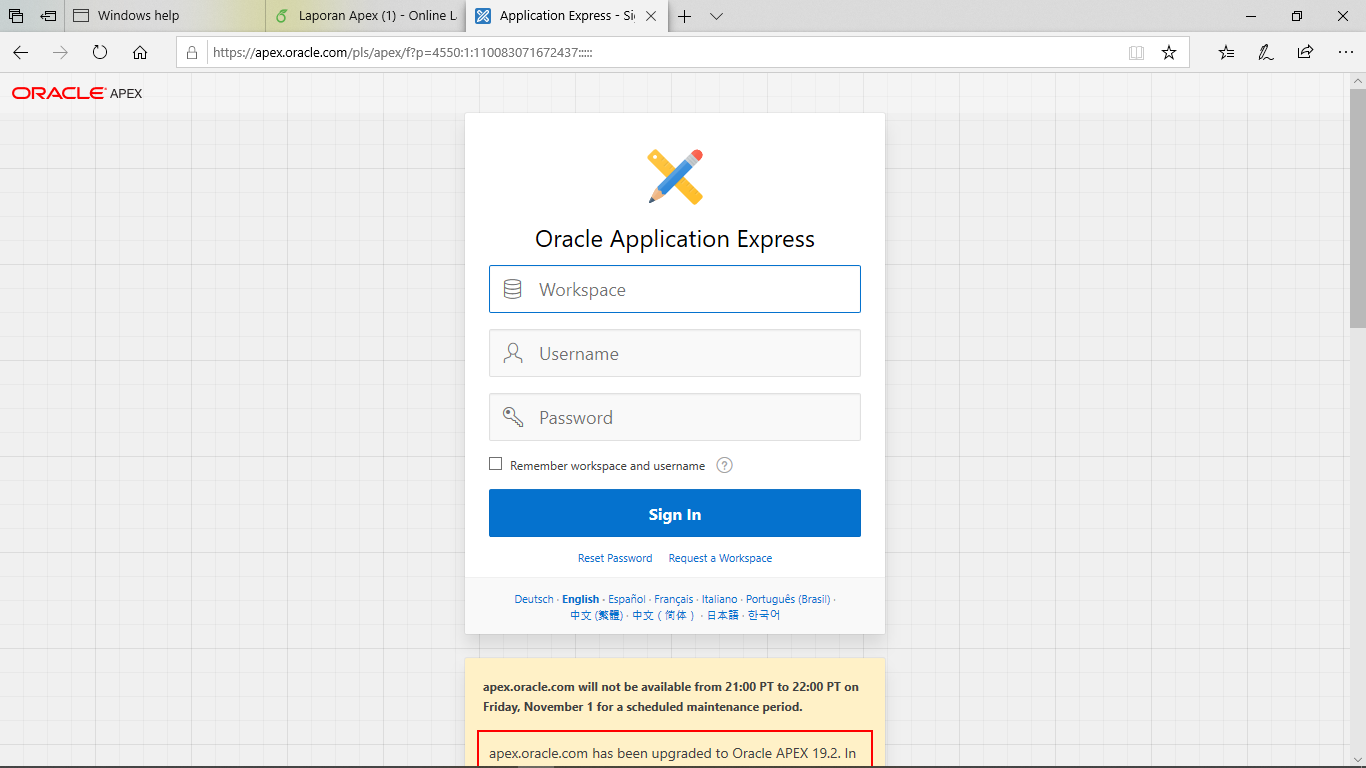
\includegraphics[scale=0.2]{figures/000.png}
    \caption{\textit{Request A Workspace.}}
    \end{center}
    \end{figure}
\begin{figure}[!htbp]
\item[3]Isikan data diri anda seperti nama,email,dan workspace.

    \begin{center}
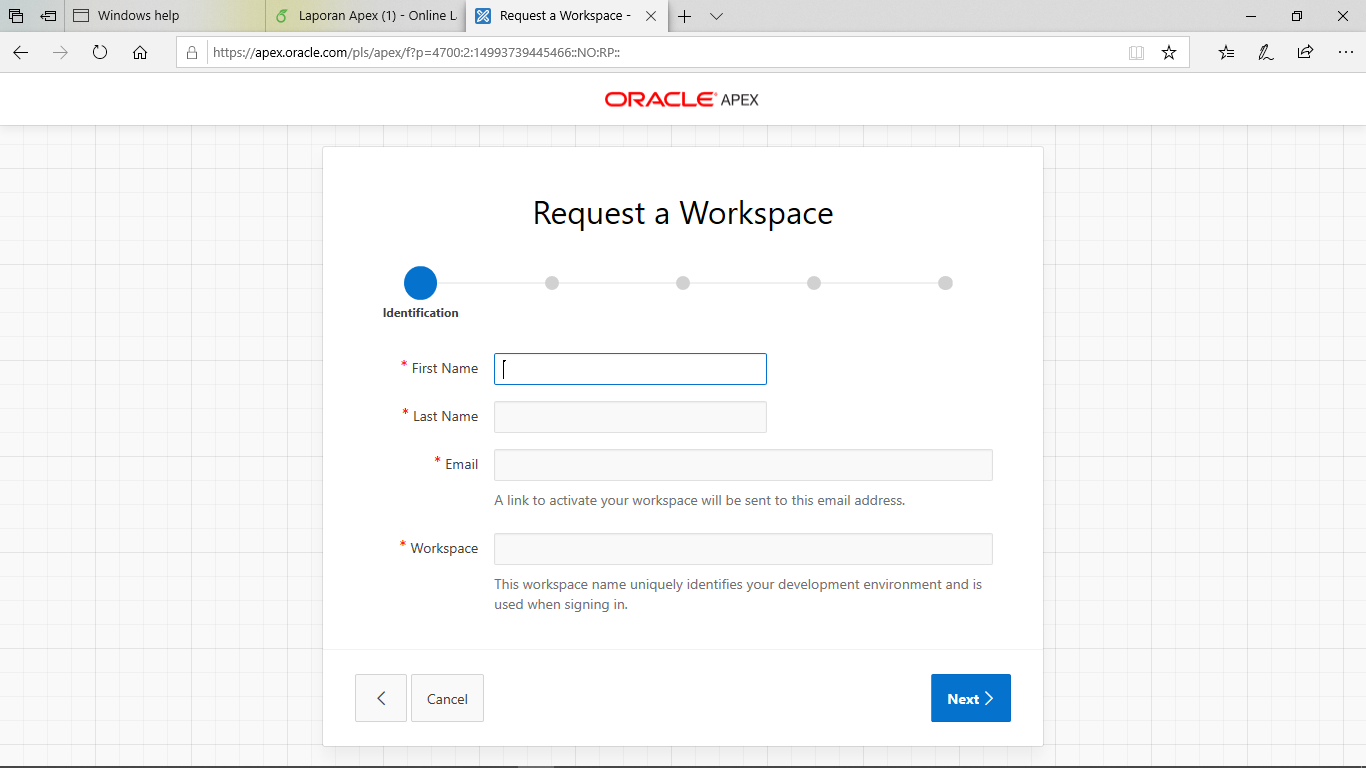
\includegraphics[scale=0.2]{figures/001.png}
    \caption{\textit{Data Diri.}}
        \end{center}
        
\item[4]Centang apakah anda pernah melakukan hal tersebut lalu next.  

    \begin{center}
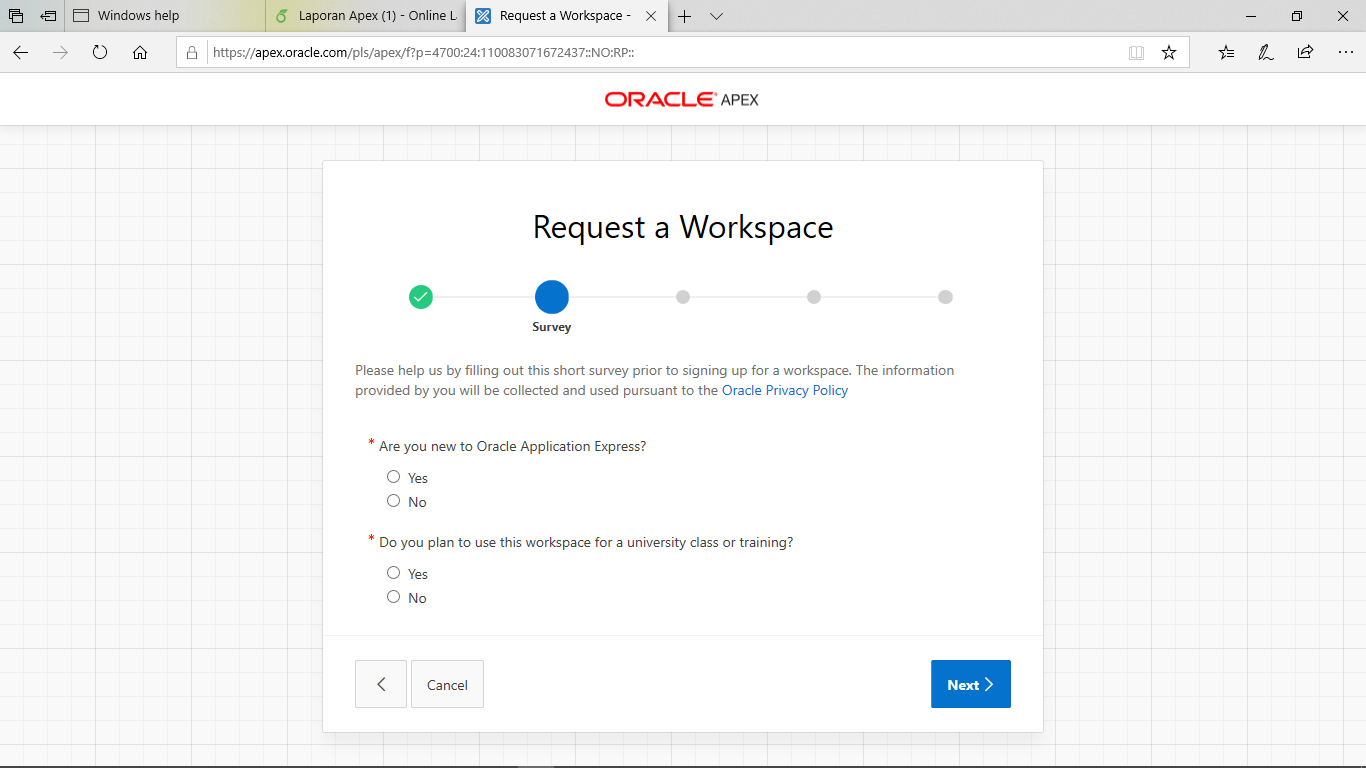
\includegraphics[scale=0.2]{figures/002.png}
    \caption{\textit{Data Diri 2.}}
        \end{center}
        \end{figure}
\begin{figure}
\item[5]Isikan pada kolom tersebut bebas, mengapa anda ingin menggunakan layanan ini ?, lalu klik next.

    \begin{center}
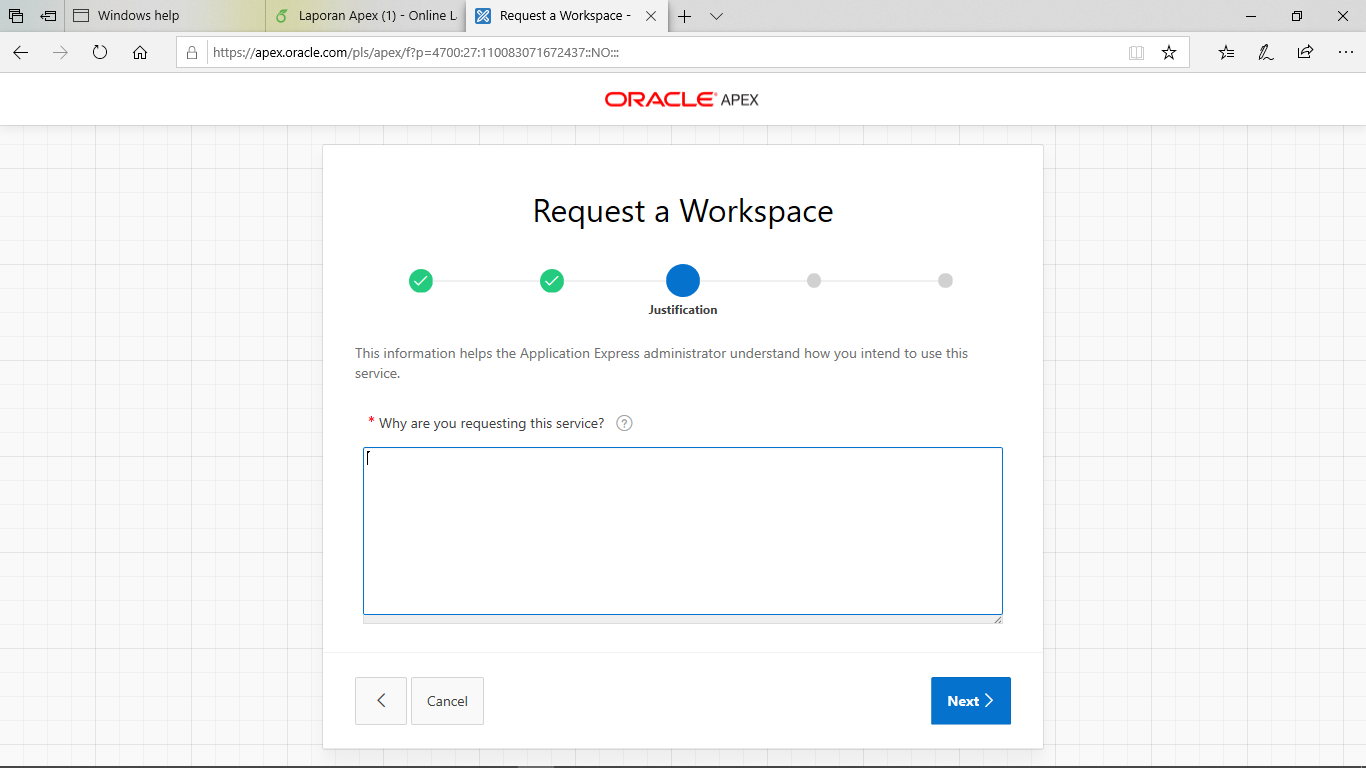
\includegraphics[scale=0.2]{figures/003.png}
    \caption{\textit{Mengapa anda memakai oracle ?.}}
        \end{center}

\label{gambar}
\end{figure}

\begin{figure}
\item[6] Centang Accept, lalu klik next.

    \begin{center}
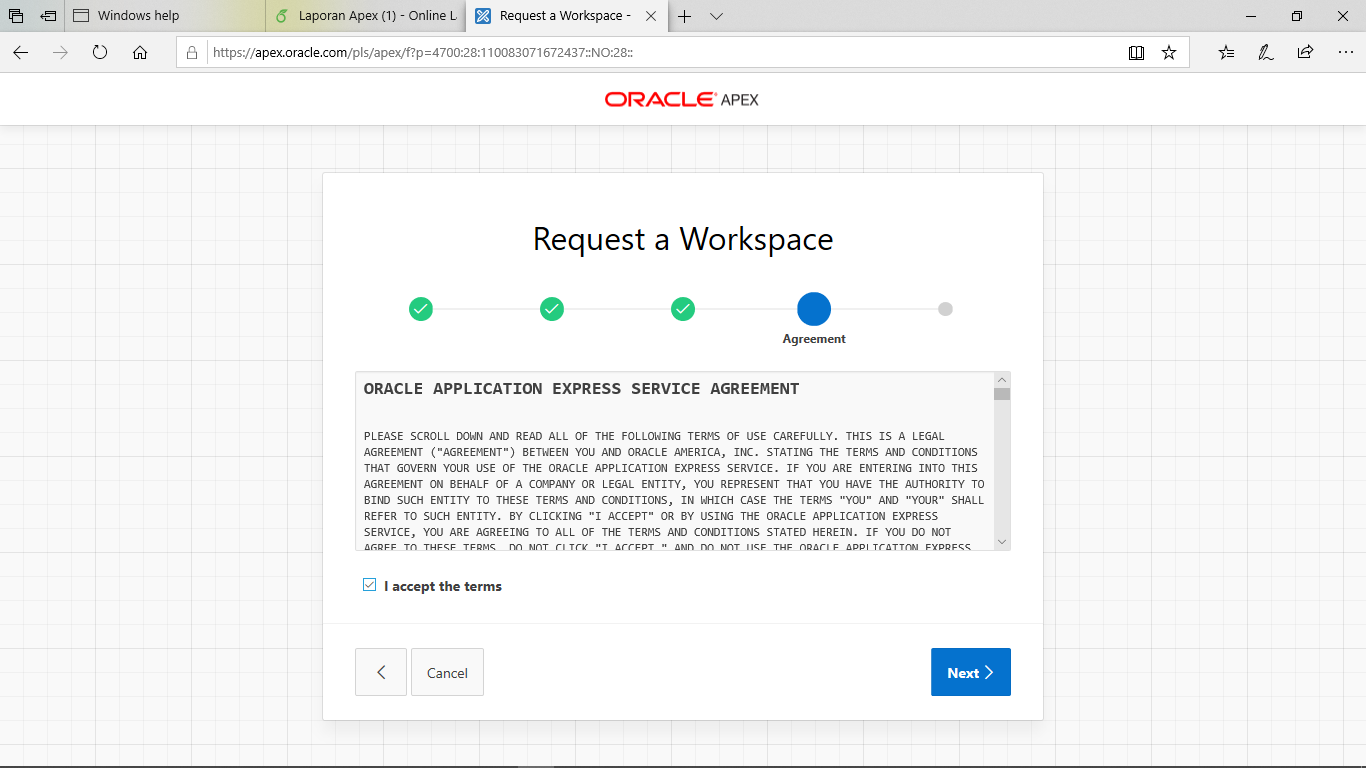
\includegraphics[scale=0.2]{figures/004.png}
    \caption{\textit{Peringatan pengunaan.}}
        \end{center}

\label{gambar}
\end{figure}

\begin{figure}
\item[7] Tahapan terakhir untuk mengkonfirmasi apakah ini anda, lalu klik next.

    \begin{center}
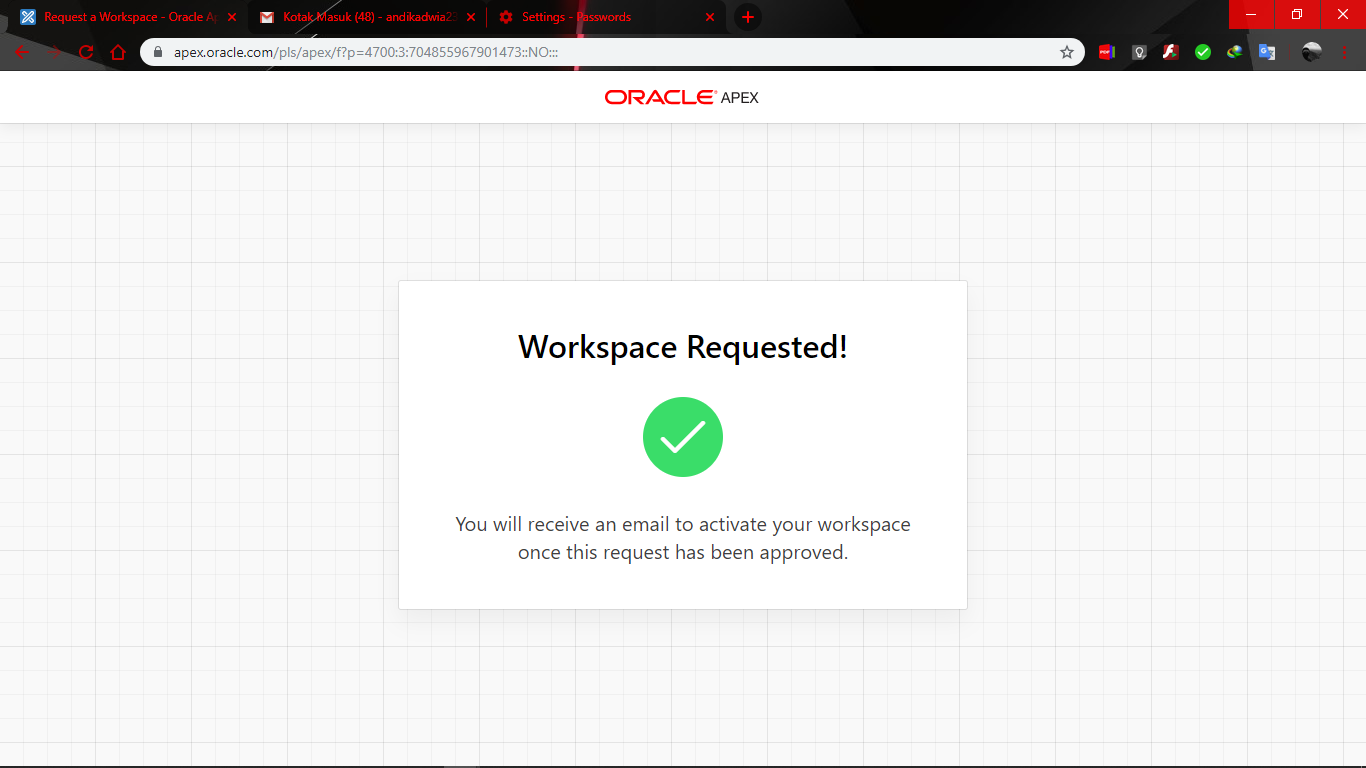
\includegraphics[scale=0.2]{figures/005.png}
    \caption{\textit{Konfirmasi.}}
        \end{center}
\label{gambar}
\end{figure}

\begin{figure}
\item[8] Finish, lalu lihat email anda.

    \begin{center}
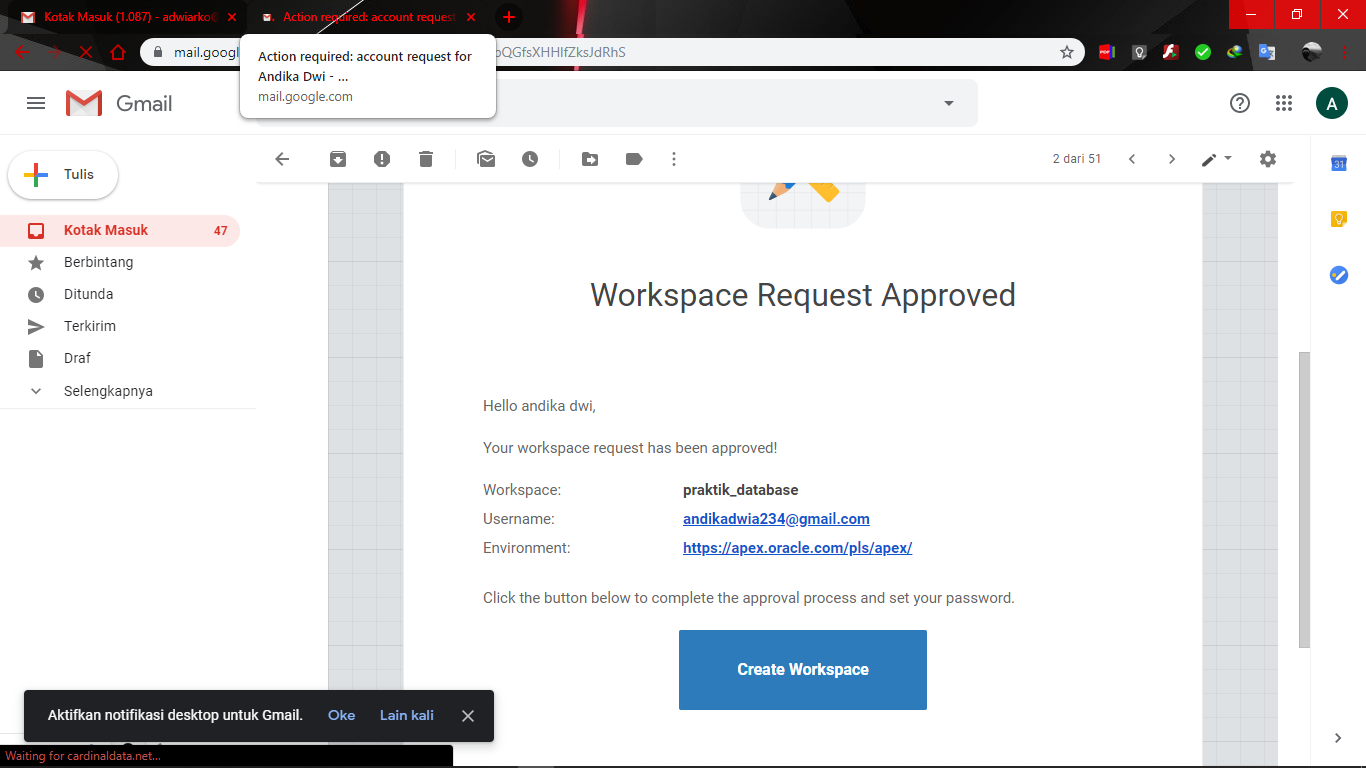
\includegraphics[scale=0.2]{figures/006.png}
    \caption{\textit{Sukses Cek Email.}}
        \end{center}
\label{gambar}
\end{figure}

\begin{figure}
\item[9] Selamat Workspace anda telah dibuat.


\label{gambar}
\end{figure}

\begin{figure}
\item[10] Workspace kamu telah dibuat lalu lanjutkan klik sign in. Login dengan akun anda dan workspace yg telah dibuat tadi.

    \begin{center}
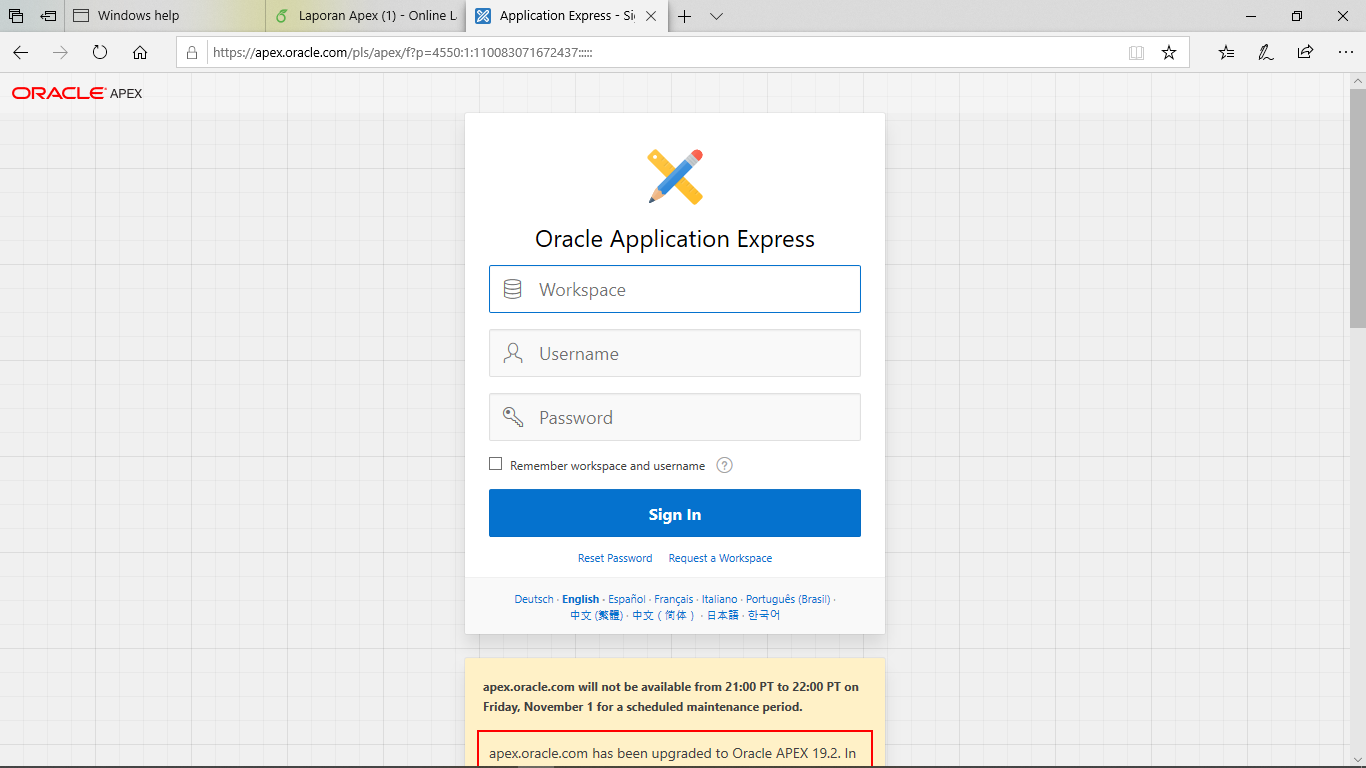
\includegraphics[scale=0.2]{figures/000.png}
    \caption{\textit{Sign In Oracle APEX.}}
        \end{center}
\label{gambar}
\end{figure}

\begin{figure}
\item[11] Masuk kedalam menu database oracle APEX dan klik App Bulider .

    \begin{center}
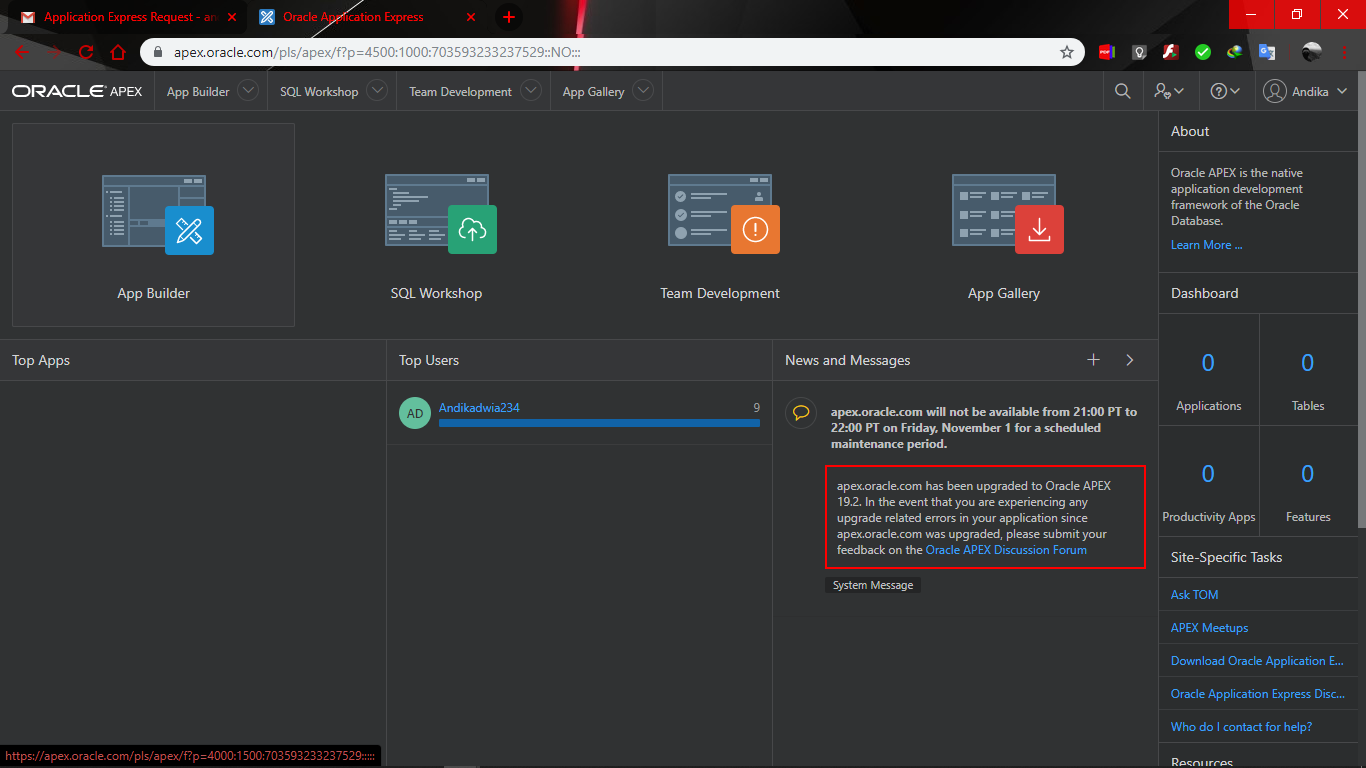
\includegraphics[scale=0.2]{figures/1.png}
    \caption{\textit{Tampilan menu oracle APEX.}}
        \end{center}
\label{gambar}
\end{figure}

\begin{figure}
\item[12] Klik create.

    \begin{center}
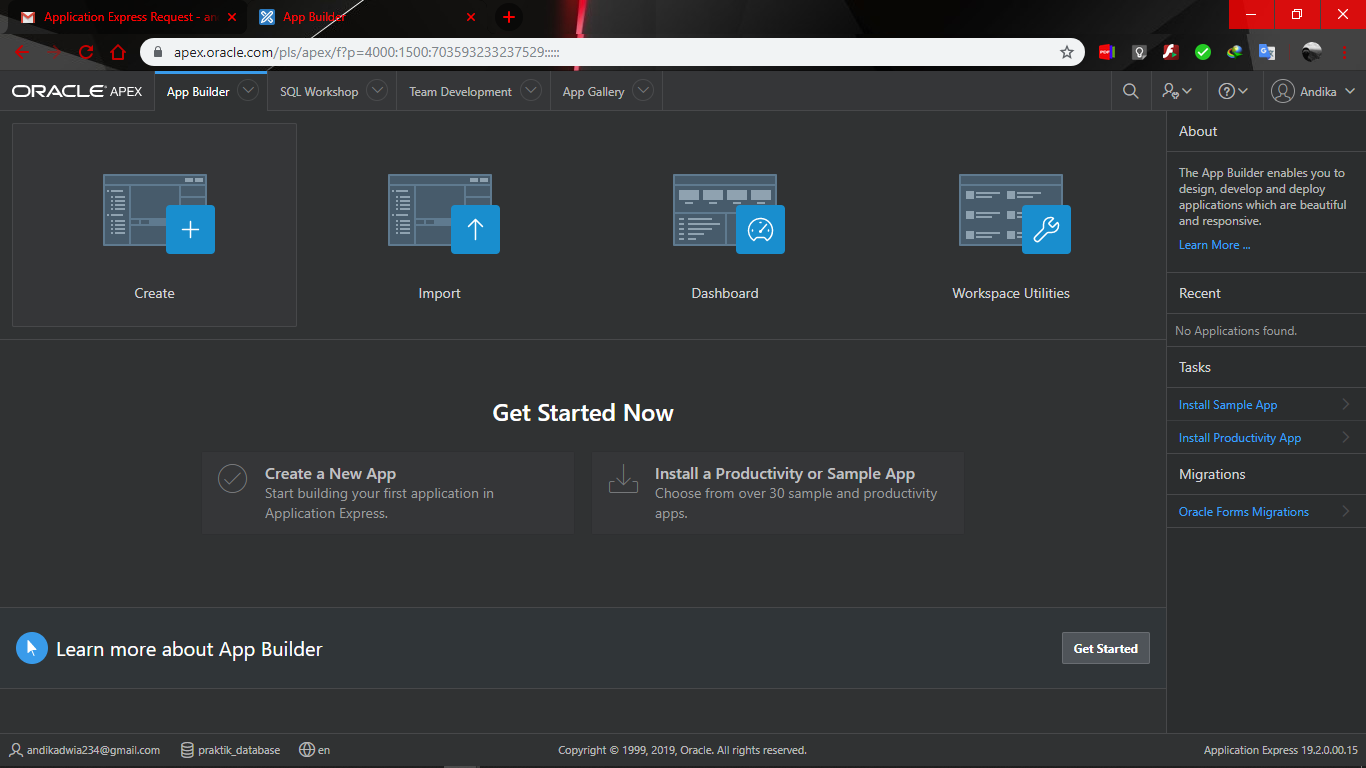
\includegraphics[scale=0.2]{figures/2.png}
    \caption{\textit{Tampilan menu APP Bulider.}}
        \end{center}
\label{gambar}
\end{figure}

\begin{figure}
\item[13] Tampilan Create New App dan pilih From A File.

    \begin{center}
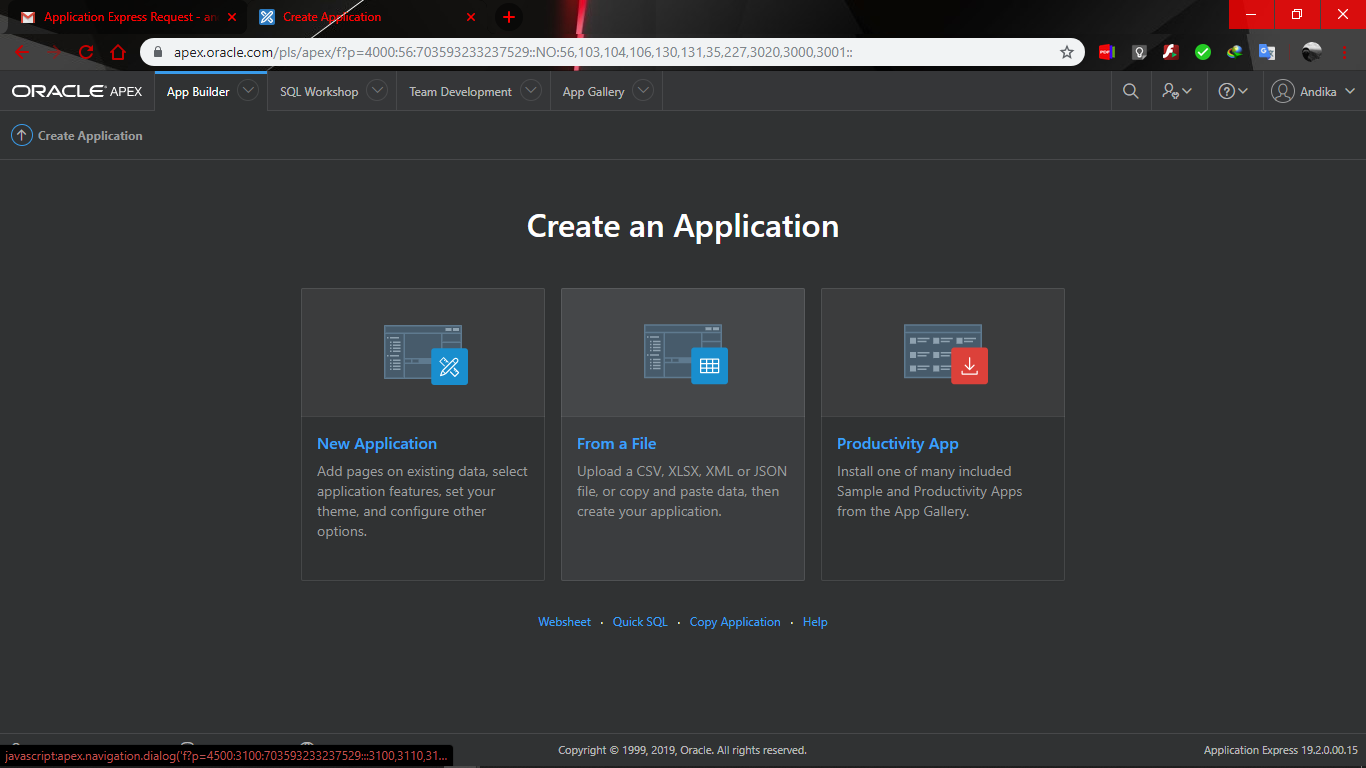
\includegraphics[scale=0.2]{figures/3.png}
    \caption{\textit{Tampilan Create}}
        \end{center}
\label{gambar}
\end{figure}

\begin{figure}
\item[14] Pilih File yang akan di inputkan ke dalam aplikasi.

    \begin{center}
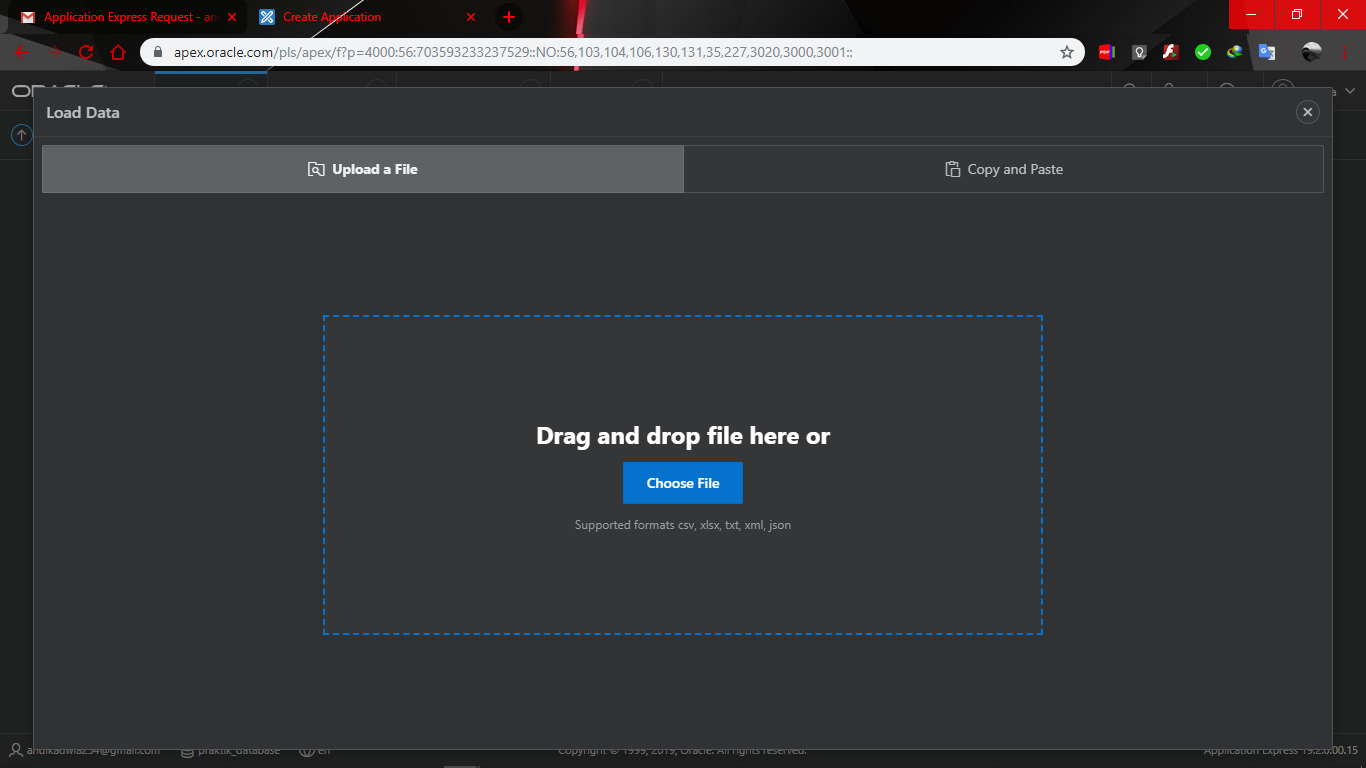
\includegraphics[scale=0.2]{figures/4.png}
    \caption{\textit{Tampilan Input File.}}
        \end{center}
\label{gambar}
\end{figure}

\begin{figure}
\item[15] Scroll ke bawah lalu setting Table Owner,Table Name,Error Table Name, dan Primary Keys, seperti gambar berikut.

    \begin{center}
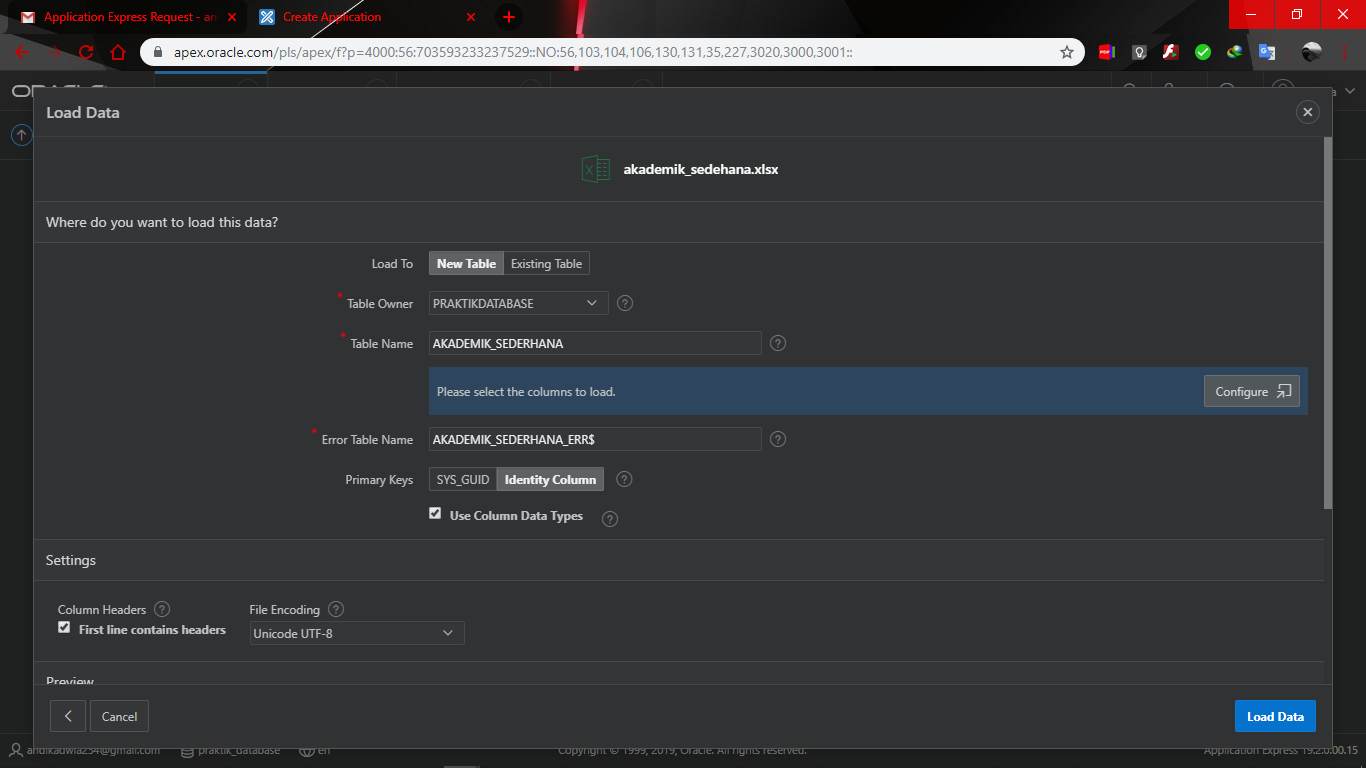
\includegraphics[scale=0.2]{figures/5.png}
    \caption{\textit{Load Data.}}
        \end{center}
\label{gambar}
\end{figure}

\begin{figure}
\item[16] Load data.

    \begin{center}
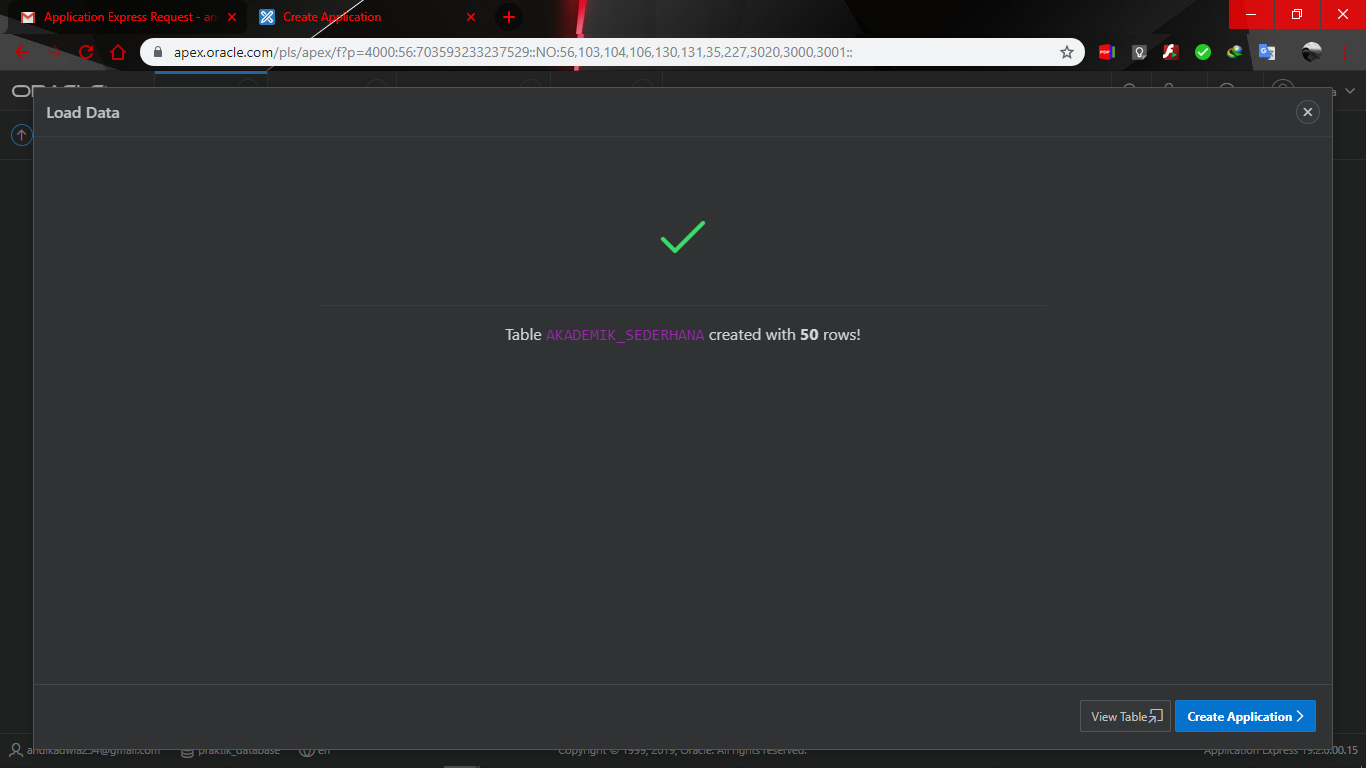
\includegraphics[scale=0.2]{figures/6.png}
    \caption{\textit{Load Data sukses.}}
        \end{center}
\label{gambar}
\end{figure}

\begin{figure}
\item[17] Kemudian, scroll kebawah dan Check All dan Create Application. 

    \begin{center}
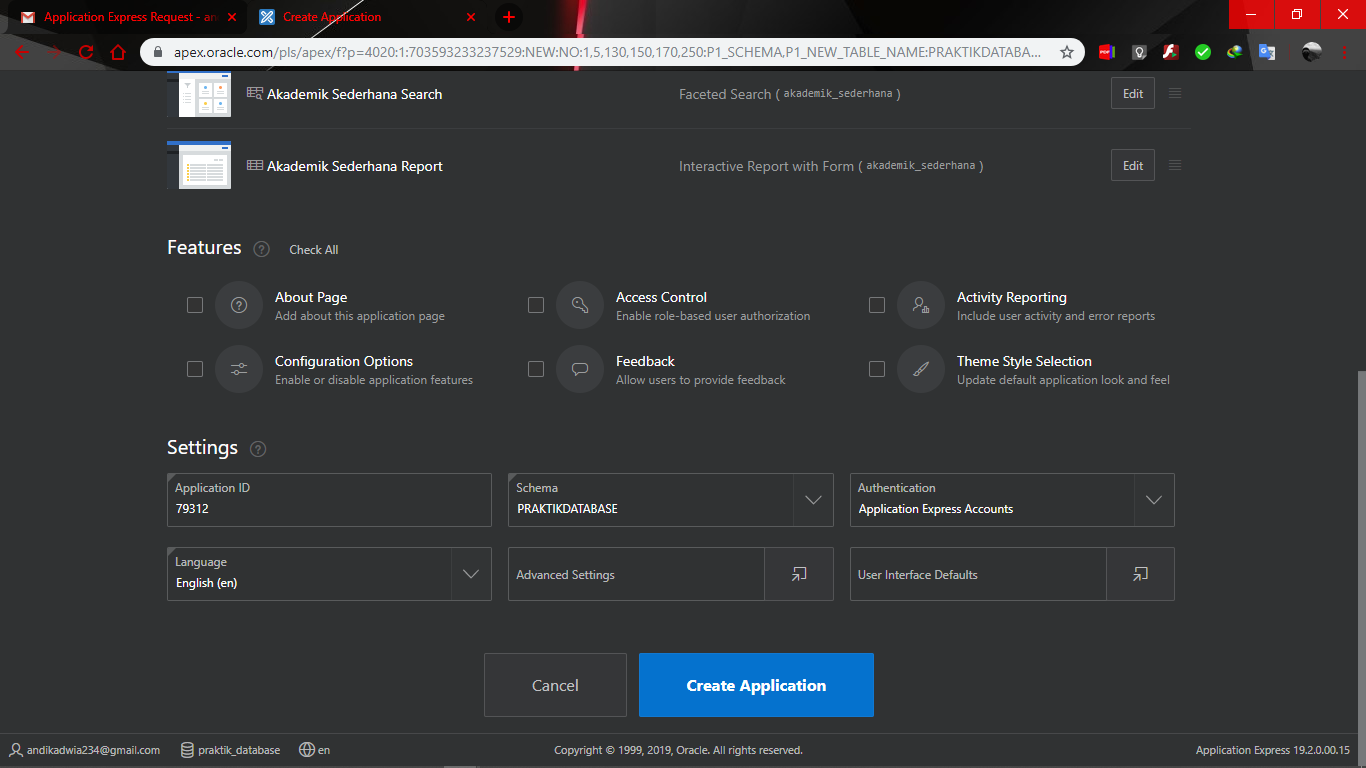
\includegraphics[scale=0.2]{figures/7.png}
    \caption{\textit{Load Data.}}
        \end{center}
\label{gambar}
\end{figure}

\begin{figure}
\item[18] Kemudian Run Application.

    \begin{center}
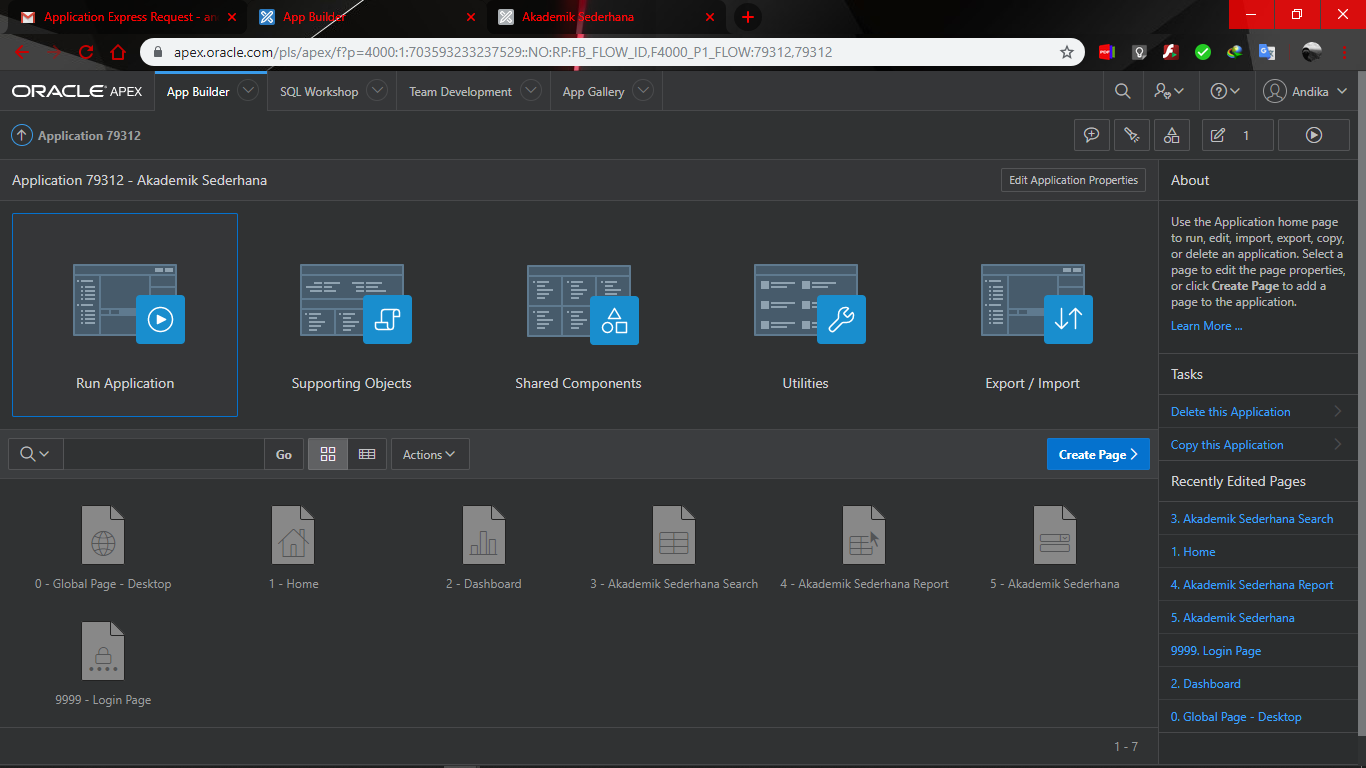
\includegraphics[scale=0.2]{figures/8.png}
    \caption{\textit{Tampilan Menu App Builder.}}
        \end{center}
\label{gambar}
\end{figure}


\begin{figure}
\item[19]Masukkan username dan password.
\item[] Username : andikadwi234@gmail.com
\item[] Password : dwi1184097
\item[] Link : https://apex.oracle.com/pls/apex/f?p=79312:1:9344647582233:::::

    \begin{center}
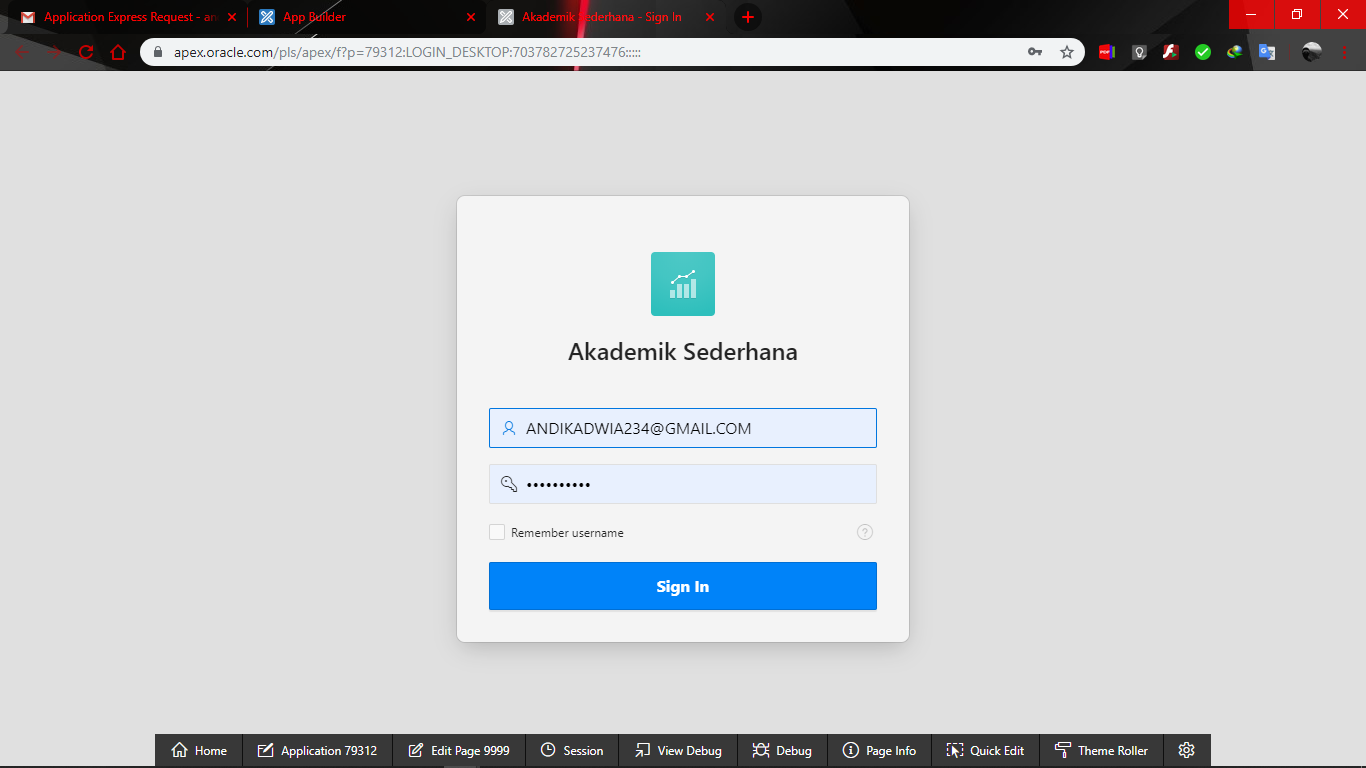
\includegraphics[scale=0.2]{figures/01.png}
    \caption{\textit{Login application.}}
        \end{center}
\label{gambar}
\end{figure}

\begin{figure}
\item[20]Tampilan Aplication .

    \begin{center}
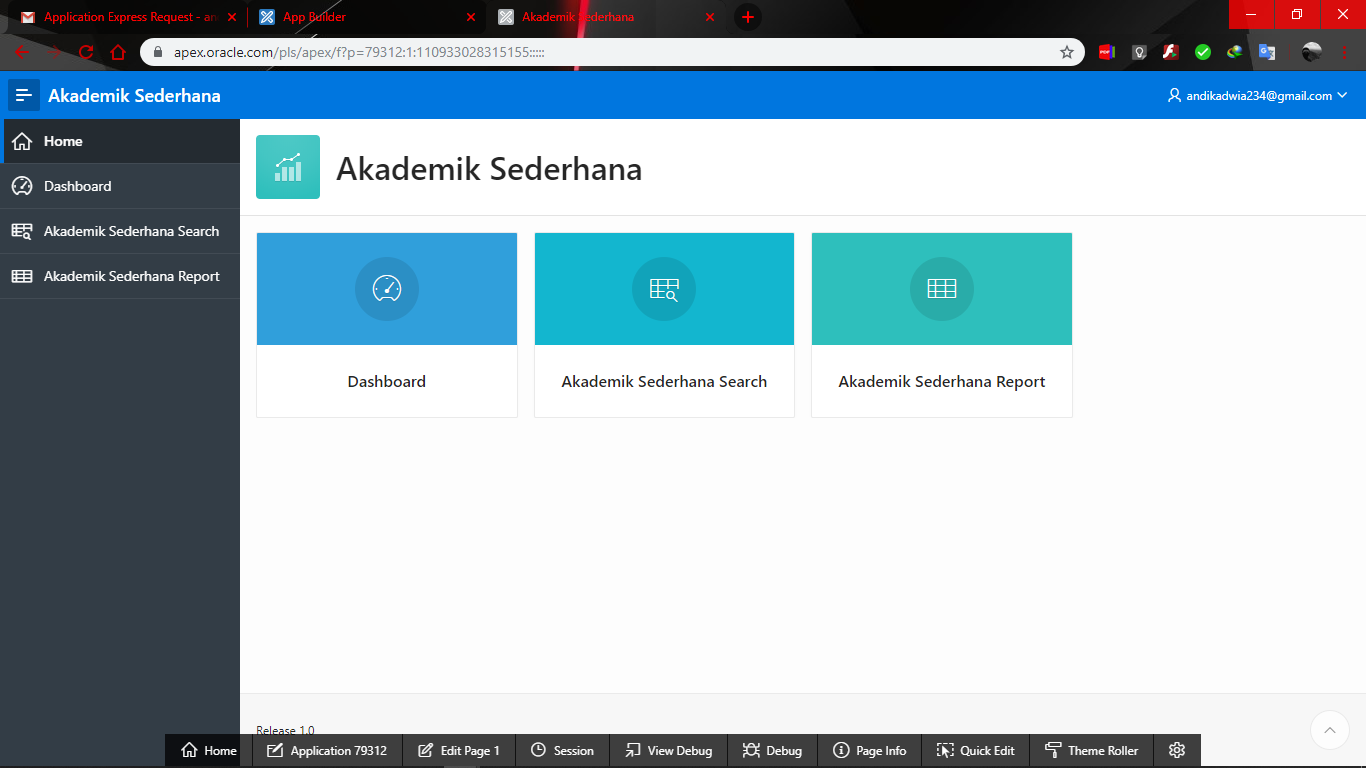
\includegraphics[scale=0.2]{figures/02.png}
    \caption{\textit{Menu Application.}}
        \end{center}
\label{gambar}
\end{figure}

\begin{figure}
\item[21]Tabel data.
    \begin{center}
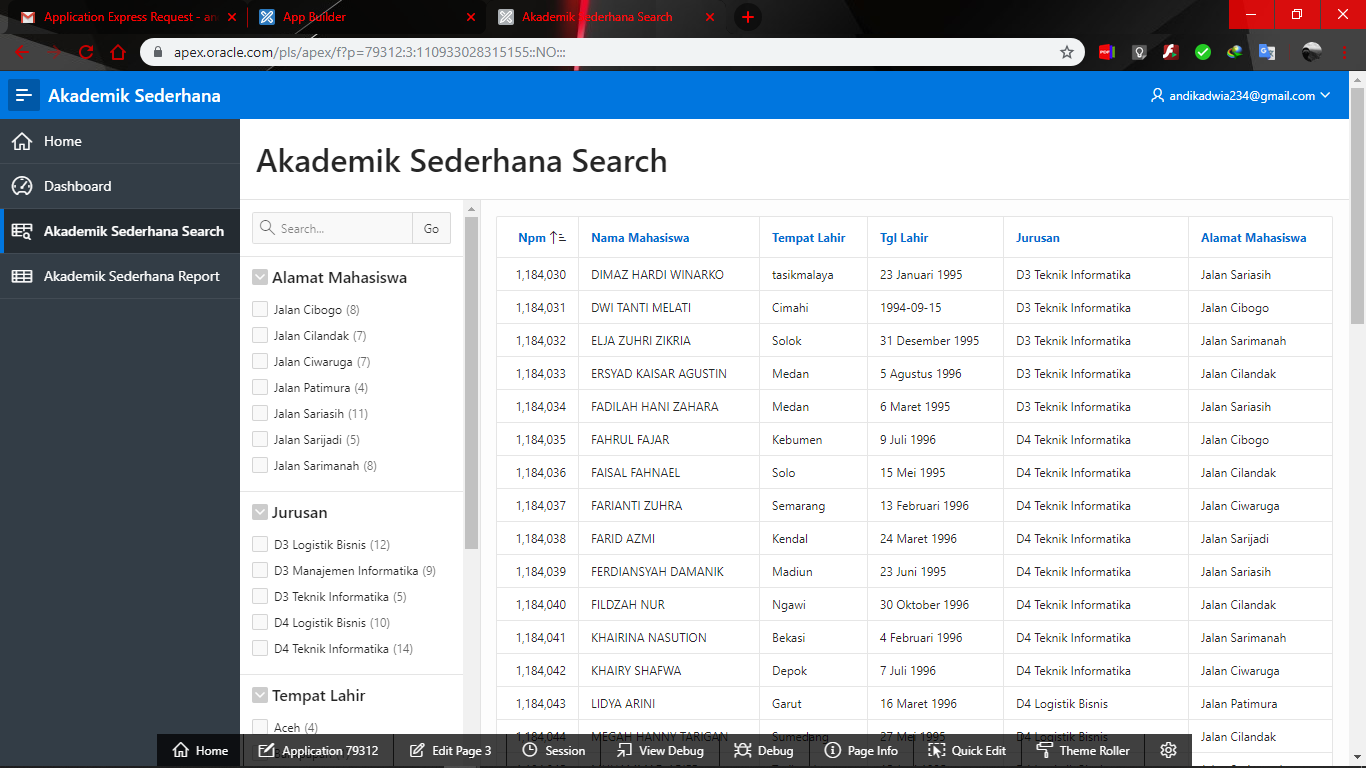
\includegraphics[scale=0.2]{figures/03.png} 
    \caption{\textit{Tampilan data mahasiswa.}}
        \end{center}
\label{gambar}
\end{figure}
\end{enumerate}
